\documentclass[a4paper, amsfonts, amssymb, amsmath, reprint, showkeys, nofootinbib, twoside]{revtex4-1}
\usepackage[spanish]{babel}
\usepackage[utf8]{inputenc}
\usepackage{float}
\usepackage[colorinlistoftodos, color=green!40, prependcaption]{todonotes}
\usepackage{amsthm}
\usepackage{mathtools}
\usepackage{physics}
\usepackage{xcolor}
\usepackage{graphicx}
\usepackage[left=23mm,right=13mm,top=35mm,columnsep=15pt]{geometry} 
\usepackage{adjustbox}
\usepackage{placeins}
\usepackage[T1]{fontenc}
\usepackage{lipsum}
\usepackage{csquotes}
\usepackage[normalem]{ulem}
\useunder{\uline}{\ul}{}
\usepackage[pdftex, pdftitle={Article}, pdfauthor={Author}]{hyperref} % For hyperlinks in the PDF
%\setlength{\marginparwidth}{2.5cm}
\bibliographystyle{apsrev4-1}

\begin{document}

%El título del experimento realizado es importante.
\title{Experimento 1: Efecto Fotoelectrico}


\author{Sergio Montoya Ramírez}
\email[Correo institucional: ]{s.montoyar2@uniandes.edu.co}

%Si necesitan poner un segundo autor, deben eliminar los porcentajes (%) iniciales.
  
%\author{Second Author}
%\email{Second.Author@institution.edu}

\affiliation{Universidad de los Andes, Bogotá, Colombia.}

\date{\today} % Si lo dejan vacío no les saldrá fecha. La fecha que se muestra es del día en que se compila.

\begin{abstract}

   Cuando una placa de metal es iluminada esta produce una corriente. El objetivo de esta practica de laboratorio es medir este efecto y las relaciones que hay entre la luz con que se ilumina la placa y los electrones emitidos. Para conseguir esto, se expuso una placa de metal a luz de distintas longitudes de onda y se midio la corriente que emitio la placa despues de esto y a su vez se investigo el voltaje de frenado aumentando el voltaje en el circuito hasta que la corriente caiga a 0.5. Tras realizar esto se comprobo la teoria y se vio que la corriente era inversamente proporcional a la longitud de onda emitida.

\end{abstract}

\maketitle

\section{Introducción}
En 1887 el físico H. Hertz estaba experimentando con dos esferas conductoras. Durante este experimento una de esas esferas fue iluminada con luz ultravioleta por error y para sorpresa de Hert una descarga electrica paso entre ambas esferas.

El efecto que observo Hertz es lo que hoy se conoce como efecto foto electrico y duro varios años sin poder ser explicado teoricamente. Fue en 1905 cuando A. Einstein logro explicar el efecto fotoelectrico. Para lograr explicarlo Einstein recurrio a un concepto bastante nuevo para la epoca, los cuantos, que M. Plank habia utilizado para explicar la radiación del cuerpo negro.\cite{Unal_Moderna} Lo que hizo Einstein fue asimilar el problema a un choque inelastico entre particulas en donde la energia que se reparten estaba dado por \cite{Texto_Guia} 
\begin{align*}
   \phi + K_max = hf
\end{align*}
\begin{itemize}
   \item $k_{max}$ : Es la energia cinetica maxima  de los electrones liberados.
   \item $h=6,6260664\times10^{34}J$ es la constante de Plank
   \item $f$ : es la frecuencia del foton incidente.
   \item $\phi$ : Se denomina \textit{función del trabajo} y depende del material e indica la energia minima para desprender un electron.
\end{itemize}
\section{Metodologia}
\begin{figure}[H]
   \centering
   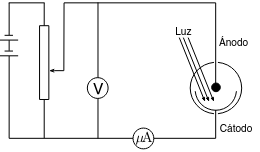
\includegraphics[scale=0.6]{Circuito.png}
   \caption{Imagen conceptual del circuito que se va a utilizar en el experimento del efecto fótoelectrico. Este circuito consiste de una fuente.La fuente esta conectada en serie con un microamperimetro (Que nos servira para captar la corriente) y en paralelo con un voltimetro. Al final de la conección y en paralelo hay tambien una separación con un Ánodo y un Cátodo que corresponde al metal que vamos a investigar. Encima de esto hay una fuente de luz que lo ilumina.}
   \label{fig:circuito}
\end{figure}
Conectamos todas las partes del circuito como se indica en la fígura \ref{fig:circuito} y revisamos que todo este funcionando bien, Para esto vamos a tapar parcialmente la luz que le puede estar llegando al espacio Ánodo/Cátodo (Por ejemplo con la mano) Luego de esto deberiamos ver una disminución de la corriente a la hora de cubrirlo. Si esto se da significa que el microamperimetro funciona. Luego de esto configuramos que el microamperimetro este en 0 para que las medidas no sean alteradas por culpa del ambiente.\cite{Guia}

A continuación, con caperuzas que cubran la luz ambiente pero que al mismo tiempo permitan iluminar con una luz concreta al Ánodo y Cátodo de esta manera vamos realizando las medidas una a una de la siguiente manera

Primero, Cubrimos con una caperuza de cierto color.Luego, iluminamos con voltaje 0 y tomamos la medida de corriente.Posteriormente aumentamos la corriente hasta que el voltaje disminuya 0.5 unidades y tomamos la medida. Por ultimo,  Repetimos hasta que se llege a 0.5 mA.

Este proceso se repite para cuantos colores se considere útil. En el experimento aqui expuesto se hace con 4 tipos de colores: Rojo (659 nm), Ámbar (590 nm), Verde (567 nm) y Azul (469 nm)
\section{Resultados y análisis}
Una vez identificados los valores experimentales se realizaron las tablas y graficas de la información obtenida. Esto con el objetivo de realizar una regresión lineal que nos permitiria hallar las pendientese intersecciones que plasmaremos en la siguiente tabla

\begin{table}
   \centering
   \caption{Tabla de datos obtenidos representados por medio de la pendiente y el punto de corte que tiene cada uno de estos una vez realizada la regresión lineal que nos indican los valores. Esta tiene tres columnas. La primera, es frecuencia cuyos datos fueron adquiridos de la guía de laboratorio \cite{Guia} y tiene como unidades nanometros. La segunda, es la pendiente de la regresión lineal realizada a los datos. Esta segunda tiene como unidades $\Omega$ dado que es una resistencia. Por ultimo, esta la Intersección de esta misma regresión lineal con el eje y. Esta columna tiene como datos $v$.}
\begin{tabular}{|c|c|c|}
   \hline
   \hline
   Frecuencia $\pm 30$& Pendiente ($\Omega$) & Intersección ($v$)\\
   \hline
   649 & $-6.2\times10^{-2} \pm 0.052$  & 0.315$\pm 0.055$\\
   590 & $-0.257\pm 0.0580 $         & 1.651$\pm 0.017$\\
   567 & $-8.6\times10^{-3} \pm 0.228 $ & 0.322$\pm 13.89$\\ 
   469 & $-7.5\times10^{-3} \pm 0.048$  & 0.718$\pm 0.975$\\
   \hline
   \hline
\end{tabular}
   \label{table:Datos}
\end{table}
Para realizar esta regresión lineal se hizo uso del lenguaje de programación python. En particular, se utilizaron las librerias Numpy y Pandas para realizar el análisis estadistico \cite{numpy.polyfit}. Para ejemplificar esto se da la siguiente imagen que es la regresión lineal del color azul.
\begin{figure}[H]
   \centering
   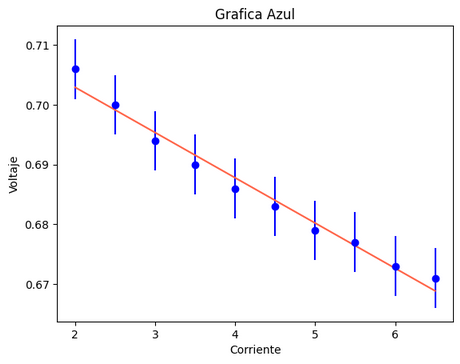
\includegraphics[scale=0.3]{Grafica_Azul.png}
   \caption{Grafica de corriente contra voltaje para el LED de color azul (es decir, 469 nm). Esta es una grafica que muestra los datos recolectados en el laboratorio, (Estos son los puntos azules) y la regresión lineal hecha con python que esta en color rojo}
   \label{fig:Azul}
\end{figure}

Por otro lado, parte de esta practica consistia en comparar los datos de un mismo color con distinta intensidad. Este apartado se realizo comparando el color amarillo con el de otro grupo. En concreto, se comparo con los datos del grupo 6 con los del grupo 4 (Al que pertenece el autor de este texto). Los resultados de esta comparación estan en la Tabla \ref{table:Camarillo} y la Grafica \ref{fig:Camarillo}
\begin{table}
   \centering
   \caption{Tabla de comparación estadistica entre los datos del grupo 4 y el grupo 6. Esta consiste de dos filas, La primera que es pendiente y tiene como unidades $\Omega$ dado que es una resistencia. La segunda, es el punto de corte con el eje Y y por tanto tiene comu unidades $v$}
   \label{table:Camarillo}
   \begin{tabular}{|c|c|c|}
      \hline
      \hline
      & Grupo 4 & Grupo 6\\
      \hline
      Pendiente $\Omega$ & -0.257$\pm 0.058$ & -0.0169$\pm 0.015$\\
      Corte $v$ & 1.651$\pm 0.017$& 0.525$\pm 0.332$\\
      \hline
      \hline
   \end{tabular}
\end{table}
\begin{figure}[H]
   \centering
   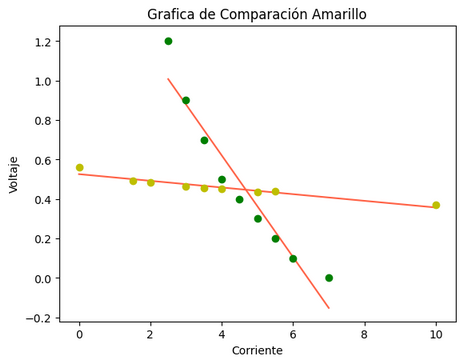
\includegraphics[scale=0.4]{Grafica_Camarillo.png}
   \caption{Figura de comparación entre el color ambar (es decir 590 nm) del grupo 4 y el grupo 6. En particular en color amarillo estan los datos obtenidos por el grupo 6 y en color verde los datos del grupo 4}
   \label{fig:Camarillo}
\end{figure}

Por ultimo, se obtuvo el dato de $k_{max}$ para esto se utilizo el punto de corte con el eje y y se multiplico por el valor absoluto de la carga del electron. Esto se hizo con el objetivo de graficarlo vs la frecuencia (que esta vez esta en Hz). El objetivo de esta grafica era conseguir la constante de plank. Dado que, esta constante es la pendiente de la grafica realizada. Con esto dicho, es importante recalcar que se retiraron los datos del color amarillo por razones que se explicaran mejor en la siguiente sección.

\begin{figure}[H]
   \centering
   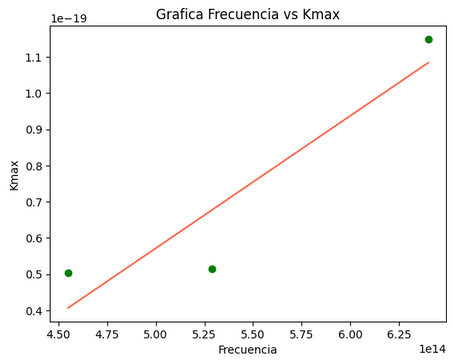
\includegraphics[scale=0.3]{Grafica_Plank.png}
   \caption{Grafica de $K_{max}$ vs Frecuencia. Para esta grafica se utilizaron los valores de frecuencia que se nos dio en la guia y para eñ vañpr de $K_{max}$ se utilizaron regresiones lineales expuestas anteriormente con lo cual llegamos a los interceptos con el eje y}
   \label{fig:Azul}
\end{figure}

Para complementar esta información la tabla \ref{table:Plank} contiene los datos estadisticos que nos interesan.
\begin{table}
   \centering
   \caption{Tabla de datos estadisticos de la grafica de $k_{max}$ vs Frecuencia, En esta estan simplemente la pendiente Experimental y Teorica. Sus unidades son $J\cdot s$. Se obtuvieron por medio de un análisis estadistico con la libreria Numpy y por medio de la guia de trabajo \cite{Guia}}
   \label{table:Plank}
   \begin{tabular}{|c|c|}
      \hline
      \hline
      &Pendiente $Js$\\
      \hline
      Experimentales&$3.66\times 10^{-34}\pm 5.29\times 10^{-29}$ \\
      Teoricos & $6.6260664\times 10^{-34}$\\
      \hline
      \hline
   \end{tabular}
\end{table}
\section{Conclusiones}
Se trabajo con 4 laceres distintos. Para cada uno de estos se realizo un análisis estadistico por medio de python y sus librerias Pandas y Numpy. Esto tenia el objetivo de encontrar para cada uno una pendiente y voltaje de frenado (que es el punto de corte con el eje y). Notese de la tabla \ref{table:Datos} que todos los voltajes de frenado son positivos y que si no contamos con el punto de corte del color ambar la longitud de onda esta inversamente relacionada con el punto de corte como lo esperabamos de manera teorica. La razon para ignorar los resultados amarillos es que los instrumentos usados a la hora de tomar los datos presentaron fallas. Tales como, la intermitencia de los LED y el fallo del voltimetro. Es importante recalcar, que el amarillo fue el ultimo color en tomarse los datos y que estos errores no se presentaron en los otros colores. Por otro lado, estas mismas razones ocasionaron que el experimento de comparación para distintas intensidades dio resultados muy distintos a los esperados. Como se puede ver en la tabla \ref{table:Camarillo} los puntos de corte difieren ampliamente siendo el punto de corte del grupo 4 aproximadamente 3 veces mayor al del grupo 6. Por ultimo, tomando en cuenta la comparación de la tabla \ref{table:Plank} podemos ver que los resultados coinciden en orden de magnitud y que el valor teorico se encuentra dentro de la incertidumbre del valor experimental. 

En conclusión, los resultados de este experimento coincidian parcialmente con lo esperado, pues aunque el color amarillo difiere ampliamente de lo que se planteaba en un inicio esto puede ser facilmente explicado por los errores a la hora de tomar datos y en consecuencia se lograron cumplir casi todos los objetivos, exceptuando el que la energia no depende de la intensidad por los errores ya planteados.
\bibliographystyle{abbrv}
\bibliography{Referencias}
\section*{Apéndice de cálculo de errores}
Para esta sección vamos indexar todas las graficas

\begin{figure}[H]
   \centering
   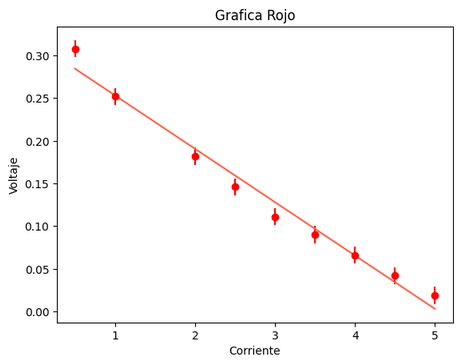
\includegraphics[scale=0.3]{Grafica_Rojo.png}
   \caption{Grafica de corriente contra voltaje para el LED de color rojo (es decir, 469 nm). Esta es una grafica que muestra los datos recolectados en el laboratorio, (Estos son los puntos rojos) y la regresión lineal hecha con python que esta en color rojo}
\end{figure}
\begin{figure}[H]
   \centering
   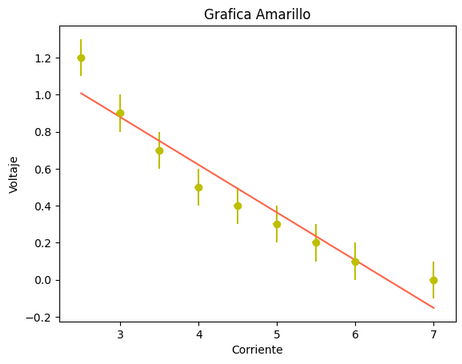
\includegraphics[scale=0.3]{Grafica_Amarillo.png}
   \caption{Grafica de corriente contra voltaje para el LED de color ambar (es decir, 469 nm). Esta es una grafica que muestra los datos recolectados en el laboratorio, (Estos son los puntos amarillos) y la regresión lineal hecha con python que esta en color rojo}
\end{figure}
\begin{figure}[H]
   \centering
   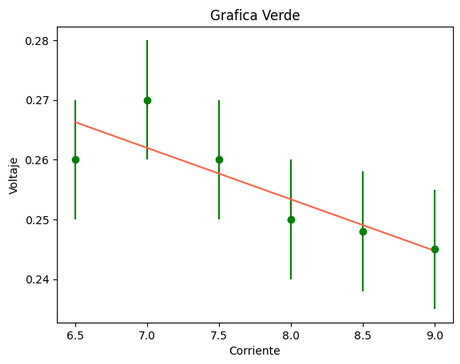
\includegraphics[scale=0.3]{Grafica_Verde.png}
   \caption{Grafica de corriente contra voltaje para el LED de color verde (es decir, 469 nm). Esta es una grafica que muestra los datos recolectados en el laboratorio, (Estos son los puntos verdes) y la regresión lineal hecha con python que esta en color rojo}
\end{figure}
\begin{figure}[H]
   \centering
   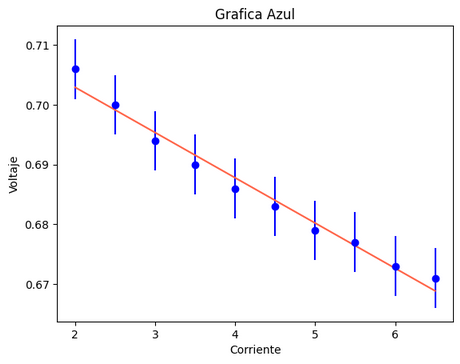
\includegraphics[scale=0.3]{Grafica_Azul.png}
   \caption{Grafica de corriente contra voltaje para el LED de color azul (es decir, 469 nm). Esta es una grafica que muestra los datos recolectados en el laboratorio, (Estos son los puntos azules) y la regresión lineal hecha con python que esta en color rojo}
\end{figure}
\end{document}
